%!TEX TS-program = xelatex
%!TEX encoding = UTF-8 Unicode

\documentclass[12pt]{article}
\usepackage{geometry}
\geometry{a4paper}
\usepackage[parfill]{parskip}
\usepackage[pdftex]{graphicx}
\usepackage{amssymb}
\usepackage[english]{babel}
\usepackage[colorlinks=true,linkcolor=blue]{hyperref}
\usepackage[official]{eurosym}

%\usepackage{fontspec,xltxtra,xunicode}
%\defaultfontfeatures{Mapping=tex-text}
%\setromanfont[Mapping=tex-text]{Hoefler Text}
%\setsansfont[Scale=MatchLowercase,Mapping=tex-text]{Gill Sans}
%\setmonofont[Scale=MatchLowercase]{Andale Mono}
\hyphenpenalty=1000

\newcommand{\swmod}[1]{\mbox{\texttt{#1}}}

\title{KINK @ NLNET}
\author{Pierpaolo Giacomin\footnote{Independent consultant.}, Mirko Rossini\footnote{CS Dept. University of Bologna.},\\Thomas Fossati and Steven Dorigotti\footnote{KoanLogic SRL.}}

\begin{document}
\maketitle
\tableofcontents
\newpage

\paragraph{Abstract}
\emph{KINK is a project which aims at bridging the ``big'' Internet with the Internet of Things by producing open standards -- mainly within the IETF CoRE Working Group -- and corresponding \mbox{opensource} implementations.}\\
\par
Figure \ref{fig:arch} illustrates the system's high-level architecture. KINK is a logical module which may reside on a standalone device or can be integrated into Customer Premise Equipment. Its function is to allow communication between HTTP, the most common Application Layer protocol of the Internet, and CoAP, a similar RESTful transfer protocol which has been designed by the IETF to be applied to particularly constrained networks such as those connecting Wireless Sensor Networks. Such generic design can find an infinite number of applications, ranging from domotics to medical, automotive and agricultural industries, only to mention a few. The diagram shows some more specific examples, such as an Energy provider gathering information from Smart Meters in a home network via the Internet $[2]$, or intelligent nodes communicating independently in a Machine 2 Machine configuration $[4]$.

\begin{center}
    \begin{figure}
        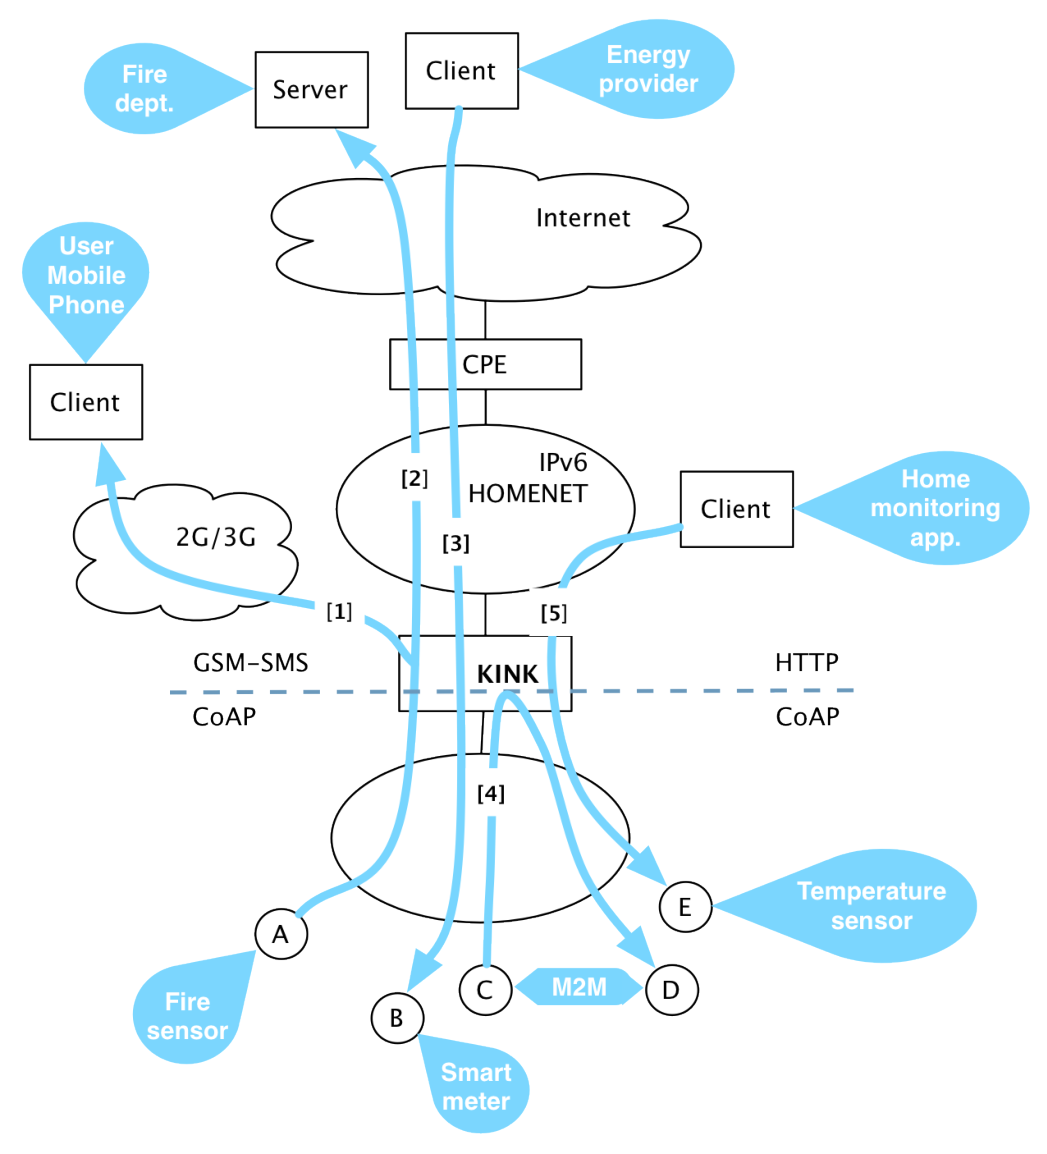
\includegraphics[width=14cm]{../share/images/kink-homenet}
            \caption{KINK architecture}
            \label{fig:arch}
    \end{figure}
\end{center}

The current KINK partners are: the Computer Science Department at the University of Bologna and KoanLogic SRL, an Italian company devoted to \mbox{opensource} and open standards implementation, and owner of a number of public GPL and BSD licensed tools\footnote{See \href{http://koanlogic.com}{http://koanlogic.com} and \href{https://github.com/koanlogic}{https://github.com/koanlogic} for details.}.

We are seeking financial aid to help us reach KINK's first deadline: the implementation of a proxy module to enable transparent communication between the unconstrained and constrained sides of the future Internet.

\section{Related Work}
We started by looking into a number of readily available opensource options when initially considering the assembly of the HTTP-CoAP proxy.  In this section, each of these components is briefly illustrated, and the main reasons for deciding against their adoption is discussed.

After careful analysis, the choice was made to build upon the \href{http://libevent.org}{libevent} core, since its non-blocking, event-driven architectural model was deemed ideal for the proxy architecture.  Furthermore, it provides an HTTP interface via the evhttp module, and has a built-in non-blocking DNS resolver, which could be easily extended to supply DNS-SD capabilities -- these having the greatest importance in mapping the embedded resource discovery functions of CoAP to the unconstrained \mbox{Internet}.

\subsection{libcoap}

(TODO THOMAS, visto che le stai provando)

\subsection{apache}

(TODO TBD, se avete qualcosa di pronto, come giustificazione di klone come risposta embedded al bloat di apache si puo' usare anche qui... se no posso occuparmene io)

\subsection{squid}

(TODO PIERPAOLO, visto che immagino non abbiate niente di pronto)

\subsection{Others}

se avete altri progetti open source E soprattutto non open source da aggiungere e' ottimo, pare che siano molto carogne sui related works quelli di nlnet, essendo che l'argomento principe su cui basano i loro rifiuti e' "e' uguale a quell'altro progetto, aiutate loro, etc...". 


\section{Work Items}
The bulk of current activity is centered around mapping HTTP and CoAP, the two main application protocols available on each communication segment.

The overall goal is to provide native communication between humans and things through seamless integration of physical objects into the Web platform.

The work items depicted in the following subsections are currently under active development, or are planned to start soon.

\subsection{CoAP Implementation}
The \href{https://github.com/koanlogic/webthings/tree/master/bits/evcoap}{\swmod{evcoap}} module fully implements the CoAP protocol as per \href{http://tools.ietf.org/html/draft-ietf-core-coap}{draft-ietf-core-coap-08} with server, client and proxy roles.

The deadline for this module is stringent as our participation at \href{http://www.etsi.org/plugtests/coap/coap.htm}{ETSI CoAP plugtests} is scheduled for the end of March 2012.

The module provides a C library based on the reactor pattern which builds on Niels Provos' \href{http://libevent.org}{libevent} and KoanLogic \href{http://koanlogic.com/libu}{libu}, and adds components (e.g. an embeddable resource-based file system) to ease the creation of sophisticated CoAP agents.

\subsection{HTTP-CoAP Mapping I-D}
The I-D \href{http://tools.ietf.org/html/draft-castellani-core-http-mapping}{draft-castellani-core-http-mapping} is a joint effort of \mbox{KoanLogic}, \mbox{Ericsson}, \mbox{InterDigital} and the Engineering Department at University of Padua (under the IETF CoRE Working Group umbrella), to provide the architectural and implementation guidance for a KINK-like component.

As such it represents a fundamental deliverable of the project as a whole, and at the same time it receives vital feedback from the implementation experience gained while developing the KINK software modules.

\subsection{Agnostic Caching}
The \href{https://github.com/koanlogic/webthings/tree/master/bits/kache}{\swmod{kache}} module implements a specialized cache aimed at storing informational resources, be it sensor generated data streams or a typical HTTP resource representation, in an agnostic way.  It provides the following features: 
\begin{itemize}
\item ability to plug different representation formats and discard strategies;
\item custom supervisor routine to compute access statistics and install/remove Observation relationships that optimize assets consumption (locally in the node and, globally, in the whole constrained network) while maintaining freshness of cached resources.
\end{itemize}


\subsection{Test Bed}
The \href{https://github.com/koanlogic/webthings/bits}{\swmod{sys}} Contiki and TinyOS HowTo's to setup a constrained network based on Zolertia Z1 motes (TODO Steven).


\subsection{CoAP Proxy Extensions for Sleepy Sensors I-D}
The \href{https://github.com/koanlogic/webthings/docs/}{draft-fossati-core-monitor-option}
(TODO Pierpaolo)


\subsection{HTTP-CoAP Proxy}
The only activity that has not yet begun, is the implementation of the proxy module, which constitutes the final deliverable of the KINK project. 

The related high level architectural design has been concluded as part of Mirko Rossini's MS thesis work.  The evcoap, kache, libu and libevent's evhttp modules provide fundamental building blocks that will be reused to match KINK's application logic.

\section{Expected Effort}
The effort needed to complete the KINK tasks is summarized in the following table -- the unit of measure is man/month referred to a senior resource.

\begin{center}
\begin{tabular}{|l|c|c|c|c|c|}
	\hline 
	  & Design & Development & Module Test & Integration Test & Total \\
	\hline 
	evcoap & - & 1.5 & 0.5 & - & 2 \\
	\hline
	kache & - & 1 & 0.5 & - & 1.5 \\
	\hline
	kink & 1 & 7.5 & - & 4 & 12.5 \\
	\hline
	spec (IETF) & 1 & 1 & - & - & 2 \\
	\hline
	\multicolumn{5}{|c|}{} & 18 \\
	\hline
\end{tabular}
\end{center}

The total expected cost is $18 \times 5000$\euro $= 90000$\euro. 

The KINK project is currently financed in toto by KoanLogic, which plans to further fund half of the expected remaining effort (i.e 45000\euro).

If the proposal is accepted, 15000\euro~are expected to come through the EU-financed BOOSTER project.

We are asking NLNET for a 30000\euro~funding to complete the budget.

\end{document}
